%  Typ dokumentu - článek, prezentace aj.
\documentclass[english]{article}

%  Nastaví vstupní a výstupní kódování znaků (encoding) a lokalizace
\usepackage[T1]{fontenc}
\usepackage[utf8]{inputenc}
\usepackage[english,czech]{babel}
\usepackage{icomma}
\usepackage{textcomp}
\usepackage{lmodern}

%  Formát papíru a odsazení od jeho okrajů
\usepackage[letterpaper]{geometry}
\geometry{verbose,tmargin=1.5cm,bmargin=2cm,lmargin=2cm,rmargin=2cm}

%  Umožňuje pracovat s grafikou
\usepackage{graphicx}
\usepackage{bigstrut}

%  Automaticky odsadí i první paragraf v každé sekci
\usepackage{indentfirst}

%  Umožňuje rozdělovat obsah na více sloupců
\usepackage{multicol}
\usepackage{booktabs}

%  Umožňuje používat hypertextové odkazy, nastavuje jejich barvu a
%  vlastnosti
\usepackage[unicode]{hyperref}
\hypersetup{
colorlinks=true, citecolor=blue, filecolor=blue, linkcolor=blue,
urlcolor=blue
}

%  Umožnění odstranění italiky u jednotek
\newcommand{\unit}[1]{\mathrm{#1}}

%  Formátování stránek, empty = odstraní číslování
% \pagestyle{empty}

%  Řádkování
\linespread{1.2}

%  Lepší zobrazování matematiky (rozšíření sum o \limits atd.)
\everymath{\displaystyle}
\usepackage{amsmath, amsthm, amssymb}

% Umožní psát přes \mathbb{N/R/Q/..} množiny čísel
\usepackage{amssymb}

%  Velikost fontu matematických výrazů v dokumentu lze pro danou
% základního fontu dokumentu upravit pomocí:
% \DeclareMathSizes{X}{Y}{Z}{U} kde:
% X je velikost fontu v dokumentu, pro kterou se matematika upraví
% Y je standartní velikost fontu matematiky
% Z je velikost fontu zmenšených (vnořených výrazů)
% U je velikost fontu ještě více zmenšených (vnořených výrazů).
\DeclareMathSizes{10}{10.5}{9}{9}

%  Nastaví autora, název, datum, skupinu měření apod. (můj vlastní
% příkaz, umožní znovu-použití v dokumentu)
\newcommand{\Author}{David Roesel}
\newcommand{\Coauthor}{Tereza Schönfeldová}
\newcommand{\Institute}{FJFI ČVUT v Praze}
\newcommand{\Subject}{FYZIKÁLNÍ PRAKTIKUM I}
\newcommand{\Group}{7}
\newcommand{\Circle}{ZS 5}
\newcommand{\Title}{Úloha \#1 \\Cavendishův experiment}
\newcommand{\Date}{15.11.2013}

% Začátek dokumentu - Formátování na výstup
\begin{document}

% Interní proměnné, možno zobrazovat u prezentací, používají se při
% generování pomocí \titlepage apod.
\author{\Author}
\title{\Title}
\date{\Date}

%  Lokalizace některých názvů do češtiny
\renewcommand{\figurename}{Obr.}
\renewcommand{\tablename}{Tab.}
\renewcommand{\refname}{Reference}

% --- Hlavička dokumentu -----------------------------------------------

\setlength{\parindent}{0cm}
\begin{multicols}{2}
\textbf{\Subject \\
        \Institute \\[0.1cm]
%\large  \Title \\[0.5cm]
\Title \\[0.5cm]
}
\begin{tabular}{rlrl}
\large Datum měření: & \Date & \large Skupina: & \Group \\
\large Jméno: & \Author & \large Kroužek:  & \Circle\\
\large Spolupracovala: & \Coauthor &\large Klasifikace:\\
\end{tabular}

\begin{flushright}

\includegraphics[scale=0.28]{../../_meta/fjfi_standart.pdf}
\hspace{0.2cm}
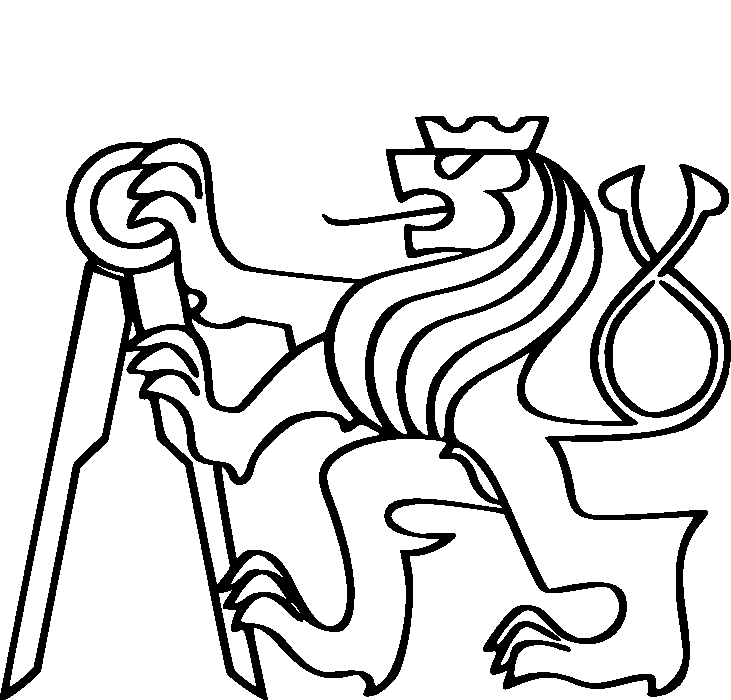
\includegraphics[scale=0.28]{../../_meta/cvut_standart.pdf}
\end{flushright}
\end{multicols}
\hrule
\vspace{0.5cm}

% ----------------------------------------------------------------------


% --- Tělo dokumentu ---------------------------------------------------
\setlength{\parindent}{0.5cm}

\section{Pracovní úkoly}

	\begin{enumerate}
		\item V přípravě odvoďte vztah pro maximální odhad relativní chyby měření $G$. Potřebné informace najdete na \emph{http://praktikum.fjfi.cvut.cz/documents/chybynav/chyby-o.pdf} na straně 1 až 4.
		\item Ve spolupráci s asistentem zkontrolujte, zda je torzní kyvadlo horizontálně vyrovnané.
		\item Dynamickou metodou změřte časový průběh torzních kmitů v jedné poloze, potom umístěte velké koule $m_{1}$ do polohy II a změřte časový průběh v této druhé poloze. U každého měření si poznamenejte i chybu tohoto měření, kterou odhadnete (čím rychleji se světelná značka pohybuje, tím větší bude chyba určení její polohy).
		\item Naměřenou závislost nafitujte funkcí (\ref{eq:fitfce}) ve vhodném programu (kupříkladu Gnuplot) a vykreslete graf naměřených dat včetně odchylek a nafitované funkce.
		\item Z výsledku fitu a naměřených hodnot spočtěte gravitační konstantu G i s výslednou chybou měření, kterou spočtěte z Vámi odvozeného vztahu z přípravy (úkol 1). Většina fitovacích programů uvádí parametry funkce i s jejich chybou - tuto chybu potom považujte za chybu měření a dosazujte ji do odvozeného vztahu.
		\item Výsledek měření gravitační konstanty $G$ srovnejte s tabulkovou hodnotou $G_t$ a ověřte, jestli se tabulková hodnota vejde do intervalu \emph{naměřená hodnota} $\pm$ \emph{chyba měření}.
	\end{enumerate}
	
\section{Vypracování}

	\subsection{Použité přístroje}
		Torzní kyvadlo, zemnící kabel, He-Ne laser, ochranné brýle (modré), podstavec pod laser, stopky, mobilní telefon, svinovací metr.
	
	\subsection{Teoretický úvod}
		\subsubsection{Gravitační konstanta}
			S gravitační silou se setkáváme neustále. Gravitační síly mají přitažlivý charakter, působí na všechny hmotné částice a Isaac Newton pro ně formuloval zákon 
			\begin{equation}\label{gravity}
			F=G \frac{m_{1}m_{2}}{r^2},
			\end{equation}
			kde $F$ je velikost gravitační síly a $m_1$, $m_2$ hmotnosti těles, mezi kterými tato síla působí. Pomocí torzního kyvadla nalezl metodu vyčíslení gravitační konstanty $G$ v roce 1798 Henry Cavendish.
			
		\subsubsection{Torzní kyvadlo}
			Během torze dochází k rotačnímu pohybu jednotlivých částí lanka a k vyjádření míry zkroucení lanka stačí změřit úhel, o který se otočí jeden konec lanka v porovnání s druhým. K lanku je připevněna činka (jak je znázorněno na Obr. \ref{fig:schema_1}) sestávající ze dvou menších koulí (o hmotnostech $m_1$) a zrcátka, od kterého se odráží laserový paprsek. Pokud se k malým koulím přiloží koule větší (o hmotnostech $m_2$), vznikne v čince moment sil
			
			\begin{equation}
			\tau_{f} = 2d(F_{1}-F_{2}).
			\end{equation}
			
			Tento moment způsobí zkroucení lanka a pootočení činky a zrcátka o úhel $\theta$. To vyvolá torzní moment $\tau_t = -k\theta$, kde $k$ je konstanta zahrnující ve své hodnotě mechanické vlastnosti lanka. Pokud je systém v rovnováze, platí 
			\begin{equation}\label{odvozeni}
			\begin{aligned}
			\tau_{f}&=-\tau_{t}\\
			2d(F_{1}-F_{2})&=k\theta,\\
			\end{aligned}
			\end{equation}
			odkud se úpravami můžeme dostat ke tvaru
			\begin{equation}
			\frac{2dG m_{1}m_{2}}{b^2}(1-\beta)=k\theta, \qquad \beta = \frac{b^3}{(b^2+4d^2)^\frac{3}{2}},\\
			\end{equation}		
			přičemž $\beta$ se nazývá geometrický faktor, $G$ je gravitační konstanta a $b$, $d$ jsou vzdálenosti vyznačené na Obr. \ref{fig:schema_1}. Z Obr. \ref{fig:schema_2}a můžeme potom vykoukat další vztahy, které pro systém platí, jako například ten pro výpočet úhlu $\theta$
			\begin{equation}\label{1}
			\tan(2\theta)\simeq 2\theta = \frac{S}{2L}=\frac{|S^2-S^1|}{2L}.
			\end{equation}
			Torzní konstantu $k$ určíme z doby kyvu $T$ a ze znalosti momentu setrvačnosti činky
			\begin{equation}\label{2}
			T^2=\frac{4\pi^2I}{k}, %=\frac{8\pi^2m_{1}(d^2+\frac{2}{5}r^2)}{k},
			\end{equation}
			kde $I$ je moment setrvačnosti činky. Za použití Steinerovy věty a nakombinováním všech předchozích vzorců podle \cite{bib:zadani} dostáváme pro výpočet gravitační konstanty 
			\begin{equation}\label{G}
			G=\frac{\pi^2b^2S}{T^2m_{2}L}\frac{d^2+\frac{2}{5}r^2}{d(1-\beta)}, \qquad \beta = \frac{b^3}{(b^2+4d^2)^\frac{3}{2}}.
			\end{equation}	
		
		\subsubsection{Tlumené kmity}
			V rámci analýzy dat zjišťujeme parametry $T$ a $S$ proložením naměřených hodnot funkcí pro tlumené harmonické kmity, která má tvar 
			\begin{equation}\label{eq:fitfce}
				f(t)=Ae^{-\delta t}\sin\left(\frac{2\pi}{T^{(1, 2)}}t+\varphi \right) + S^{(1,2)}.
			\end{equation}
			
		\subsubsection{Domácí úkol}	
			Maximální odhad chyby můžeme podle \cite{bib:h3} spočítat pomocí vzorce
			\begin{equation}
				\Delta\omega = \left|\frac{\partial \omega}{\partial x}\right|\Delta x + \left|\frac{\partial \omega}{\partial y}\right|\Delta y + \ldots
			\end{equation}
			Pro náš výpočet gravitační konstanty $G$ potom pomocí
			\begin{equation}\label{eq:horni_odhad}
				\Delta G = \left|\frac{\partial G}{\partial S}\right|\Delta S + \left|\frac{\partial G}{\partial T}\right|\Delta T +  \left|\frac{\partial G}{\partial L}\right|\Delta L,
			\end{equation}
			kde $\Delta S$ je součet chyb $\sigma_{S_1}$ a $\sigma_{S_2}$, $\Delta T$ chyba spočítaná podle (\ref{eq:chyba_neprime_mereni}) z hodnot $T_1$, $T_2$ a jejich chyb a $\Delta L$ chyba $\sigma_L$.
	
	\subsection{Postup měření}
			Torzní kyvadlo jsme nevyrovnávali, jelikož nám bylo řečeno, že je vyrovnané dobře. V případě, že by nebylo, bychom to poznali na křivosti pohybu laseru po stěně a vzhledem k tomu, že se odraz laseru pohyboval pouze po měřítku, můžeme říct, že bylo vyrovnané dostatečně. Vyrovnání provádíme proto, aby na námi měřené hodnoty nemělo vliv gravitační pole Země. Dalším z externích vlivů, který jsme museli před začátkem měření eliminovat, byla možnost působení elektrostatické síly. Toho jsme dosáhli uzemněním aparatury k tomu určeným vodičem.  
			
			Během měření zaznamenáváme výchylku činky v čase a proložením funkcí pro tlumené harmonické kmity (\ref{eq:fitfce}) určíme parametry $S_1$, $S_2$, $T_1$ a $T_2$, tedy hodnoty rovnovážných poloh a period při obou dvou polohách velkých koulí. Před měřením bylo potřeba změřit vzdálenost zrcátka od stěny s měřítkem. Vlastní měření jsme prováděli podle následujícího postupu:
			
			\begin{enumerate}
			    \item Odaretujeme kyvadlo, zapneme laser a nasměrujeme ho na zrcátko tak, aby jeho odraz kmital přibližně kolem středu stupnice na protější stěně.
			    \item Kyvadlo necháme ustálit (řádově desítky minut) a ujistíme se, že v krajních polohách nedochází k odrazu činky od stěn. 
			    \item Na k tomu určené nástavce opatrně umístíme větší koule a jemně je posuneme tak, aby se dotýkaly stěn. 
			    \item Opět se ujistíme, že jsme nijak nenarušili pohyb soustavy a necháme kmity ještě chvíli ustálit.
			    \item Následně zaznamenáváme každých 20 sekund polohu odrazu laseru na měřítku po dobu zhruba 25 minut.
			    \item Po naměření hodnot přesuneme těžší koule do druhé polohy a opakujeme předchozí dva body.
			\end{enumerate}
			
			Chybu každé naměřené hodnoty určíme z okamžité rychlosti tečky laseru jako dráhu, kterou při ní mohl urazit, za čas, jaký trvá hodnotu odečíst a  který jsme určili přibližně na $t_{od} = 1 $ s.
		
	\subsection{Naměřené hodnoty}
		Naměřené hodnoty jsou uvedeny v Tab. \ref{tab:1} a vyneseny do grafů na Obr. \ref{fig:g_1} a \ref{fig:g_2}. V tabulce kromě naměřených hodnot uvádíme hodnoty ze zadání \cite{bib:zadani}, které bereme jako absolutně přesné konstanty. Z těchto zadaných a naměřených hodnot jsme pak podle (\ref{G}) určili gravitační konstantu s horním odhadem chyby (\ref{eq:horni_odhad}) jako
		\begin{equation}
		G = (6,4 \pm 0,6)\ \unit{\cdot 10^{-11}\ N\cdot m^2\cdot kg^{-2}}.
		\end{equation}
		
		\begin{table}[h]
		\begin{center}
		
		\begin{tabular}{cccccc}
		\toprule
		$r$ [mm] & $d$ [mm] & $b$ [mm] & $m_2$ [kg] &	$\beta$ [-]& $L \pm \sigma_L$ [m] 		\\ \midrule
		9,55   	 & 50,7    	& 45  	   & 1,24  	    & 0,066744     & $6,00 \pm 0,05$ 	\\
		\midrule&&&&&\\  &&&&&\\ \midrule
		      $S_1 \pm \sigma_{S_1}$ [cm] 			& $S_2 \pm \sigma_{S_2}$ [cm]  		& $S \pm \Delta_S$ [cm]			& $T_1\pm\sigma_{T_1}$ [s] 		& $T_2\pm\sigma_{S_2}$ [s] & $T\pm\Delta_T$ [s] \\ \midrule
			 $104,2 \pm 0,8$ 	& $114,9 \pm 0,2 $ 	& $10,7 \pm  0,8$ 	& $498,4 \pm 0,4$ 	& $ 499 \pm 3$  & $499 \pm 2$\\
		\bottomrule
		\end{tabular}%
		\caption{Tabulka zadaných a naměřených hodnot; $r$, $d$, $b$ a $m_2$ jsou zadané hodnoty \cite{bib:zadani}, $\beta$ je z nich vypočítaná konstanta, $L \pm \sigma_L$ je vzdálenost zrcátka od měřítka na stěně, $S$, $\Delta_{S}$ rozdíl rovnovážných poloh $S_1$ a $S_2$ se svou chybou a $T$, $\Delta_T$ perioda kmitů se svou chybou spočítaná jako průměr $T_1$ a $T_2$.}
		\label{tab:1}
		\end{center}
		\end{table}			
	
	\subsection{Diskuse}
		Nejméně přesným článkem celého měření bylo asi určování vzdálenosti zrcátka od měřítka na stěně. Vzhledem k tomu, že byl svinovací metr dlouhý pouze pět metrů a vzdálenost ke stěně se pohybovala kolem šesti, bylo nutné použít připravený provázek. Měření jsme prováděli podél stěny, ale provázek nebyl pravděpodobně dokonale napnut, nekončil přesně na úrovni zrcátka a jeho překládáním mohlo dojít k dalším chybám. Stěna, podél které jsme měřili, navíc také nemusela být kolmá na tu s měřítkem. 
		
		Gravitační konstanta má podle tabulek \cite{bib:tabulky} vycházet jako $G_t = (6,6738 \pm 0,0008) \unit{\cdot 10^{-11}\ N\cdot m^2\cdot kg^{-2}}$. Nám se ji podařilo určit na $G = (6,4 \pm 0,6)\ \unit{\cdot 10^{-11}\ N\cdot m^2\cdot kg^{-2}}$, což tabulkové hodnotě odpovídá. V případě, že bychom místo horního odhadu chyby (\ref{eq:horni_odhad}) použili standardní chybu nepřímého měření (\ref{eq:chyba_neprime_mereni}), tabulková hodnota by už neležela v chybovém intervalu našeho výsledku. Dá se tedy předpokládat, že docházelo k systematickým chybám. Nepřesnost výsledku mohla být způsobena nevyváženou původní pozicí aparatury, kterou jsme nekontrolovali, již zmíněným nepřesným změřením vzdálenosti zrcátka od měřítka nebo systematicky chybným odečítáním jedné sady měření ze stupnice na stěně. Výsledek by se dal dále lehce ovlivnit vybráním jiné podmnožiny výsledků z naměřených dat. 
		
\section{Závěr}
	V přípravě jsme odvodili vztah pro maximální odhad relativní chyby měření $G$. Asistent nám zaručil, že je torzní kyvadlo horizontálně vyrovnané a pak jsme dynamickou metodou změřili časový průběh torzních kmitů ve dvou různých polohách. Naměřenou závislost jsme nafitovali patřičnou funkcí (\ref{eq:fitfce}) a vykreslili jsme graf včetně odchylek (Obr. \ref{fig:g_1}, \ref{fig:g_2}). Z výsledků fitů a naměřených hodnot jsme určili gravitační konstantu i s výslednou chybou měření na $G = (6,4 \pm 0,6)\ \unit{\cdot 10^{-11}\ N\cdot m^2\cdot kg^{-2}}$. Námi změřenou hodnotu jsme pak porovnali s tabulkovou a diskutovali její správnost.
	
	
\section {Použitá literatura}
% --- Literatura a reference -------------------------------------------
\begingroup
\renewcommand{\section}[2]{}

\begin{thebibliography}{9}
\bibitem{bib:zadani} Kolektiv KF, \emph{Návod k úloze: Cavendishův experiment} [Online], [cit. \today] \newline 
http://praktikum.fjfi.cvut.cz/pluginfile.php/80/mod\_resource/content/7/Cavendish\_v1.pdf

\bibitem{bib:h3} Petr Chaloupka, \emph{Jak zpracovávat data} [Online], [cit. \today] \newline 
https://dl.dropboxusercontent.com/u/11296940/zfm/h3.pdf

%\bibitem{bib:navody} Kolektiv KF, \emph{Návody k přístrojům} [Online], [cit. \today] \newline http://praktikum.fjfi.cvut.cz/documents/chybynav/navody-o.pdf

\bibitem{bib:chyby} Kolektiv KF, \emph{Chyby měření} [Online], [cit. \today] \newline http://praktikum.fjfi.cvut.cz/documents/chybynav/chyby-o.pdf

\bibitem{bib:tabulky} J. Mikulčák a kol., Matematické, fyzikální a chemické tabulky \& vzorce. Prometheus,
Praha 2009.\newline
ISBN 978-80-7196-264-9

\end{thebibliography}
\endgroup
% ----------------------------------------------------------------------

\clearpage
\part{Přílohy}

\subsection{Domácí příprava}
	Domácí příprava je přiložena k protokolu.
%\clearpage
\subsection{Statistické zpracování dat}
	Pro statistické zpracování využíváme aritmetického průměru:
	\begin{equation} \label{eq:aritmeticky_prumer}
	\overline{x} = \frac{1}{n}\sum\limits_{i=1}^{n}x_i,
	\end{equation}
	
	jehož chybu spočítáme jako 
	\begin{equation} \label{eq:chyba_aritmetickeho_prumeru}
	\sigma_0 = \sqrt{\frac{1}{n(n-1)} \sum\limits_{i=1}^{n}\left( x_i - \overline{x} \right)^2 },
	\end{equation}
	
	kde $ x_i $ jsou jednotlivé naměřené hodnoty, $ n $ je počet měření, $ \overline{x} $ aritmetický průměr a $ \sigma_0 $ jeho chyba \cite{bib:chyby}.
	
Při nepřímém měření počítáme hodnotu s chybou dle následujících vztahů:
	\begin{equation}
	u = f(x, y, z, \ldots),
	\end{equation}
	\begin{displaymath}
	x = (\overline{x} \pm \sigma_x), \qquad
	y = (\overline{y} \pm \sigma_y), \qquad
	z = (\overline{z} \pm \sigma_z), \qquad
	\ldots,
	\end{displaymath}
	
	kde $ u $ je veličina, kterou určujeme nepřímo z měřených veličin $ x, y, z, \ldots $ 
	
	Pak
	\begin{displaymath}
	\overline{u} = f(\overline{x}, \overline{y}, \overline{z}, \ldots),
	\end{displaymath}
	\begin{equation}\label{eq:chyba_neprime_mereni}
	\sigma_u = \sqrt{\left( \frac{\partial f}{\partial x} \right)^2 \sigma^2_x + \left( \frac{\partial f}{\partial y} \right)^2 \sigma^2_y + \left( \frac{\partial f}{\partial z} \right)^2 \sigma^2_z + \ldots},
	\end{equation}
	\begin{displaymath}
	u = (\overline{u} \pm \sigma_ u).
	\end{displaymath}
	
V případě, že máme několik různě přesných měření stejné veličiny, používáme vztah pro vážený průměr:
	\begin{equation} 
	\bar{x}=\frac{\sum\limits_{i=1}^{n}p_{i}x_{i}}{\sum\limits_{i=1}^{n}p_{i}},
	\end{equation}
	
	kde $\bar{x}$ je vážený průměr, $x_{i}$ jsou jednotlivá měření a pro $p_{i}$ platí
	 
	\begin{equation}
	p_{i}=\frac{1}{\sigma_{i}^{2}},
	\end{equation}
	
	kde $\sigma_{i}$ jsou jednotlivé chyby daných měření.
	 
	Celkovou chybu tedy vypočítáme ze vztahu
	\begin{equation} \label{eq:vazeny_prumer}
	\sigma_{0}=\sqrt{\frac{1}{\sum\limits_{i=1}^{n}p_{i}}}.
	\end{equation}
	
\clearpage
\subsection{Schémata}

	\begin{figure}[h!]
			\begin{center}
			    	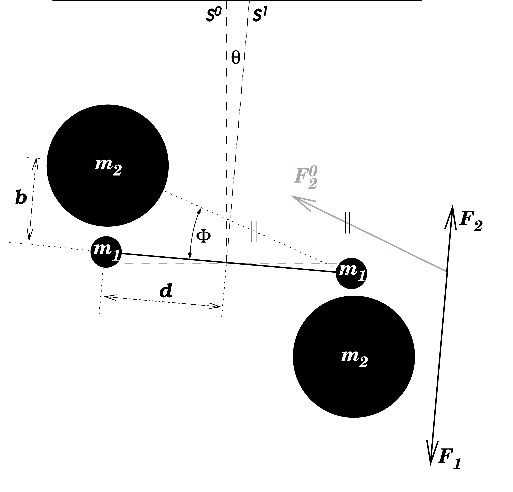
\includegraphics[width=0.7\linewidth]{att/obr1.pdf}
					\caption{Schéma zapojení z \cite{bib:zadani}.}
					\label{fig:schema_1}
						    	
					
			\end{center}
		\end{figure}
		
		\begin{figure}[h!]
				\begin{center}
				    	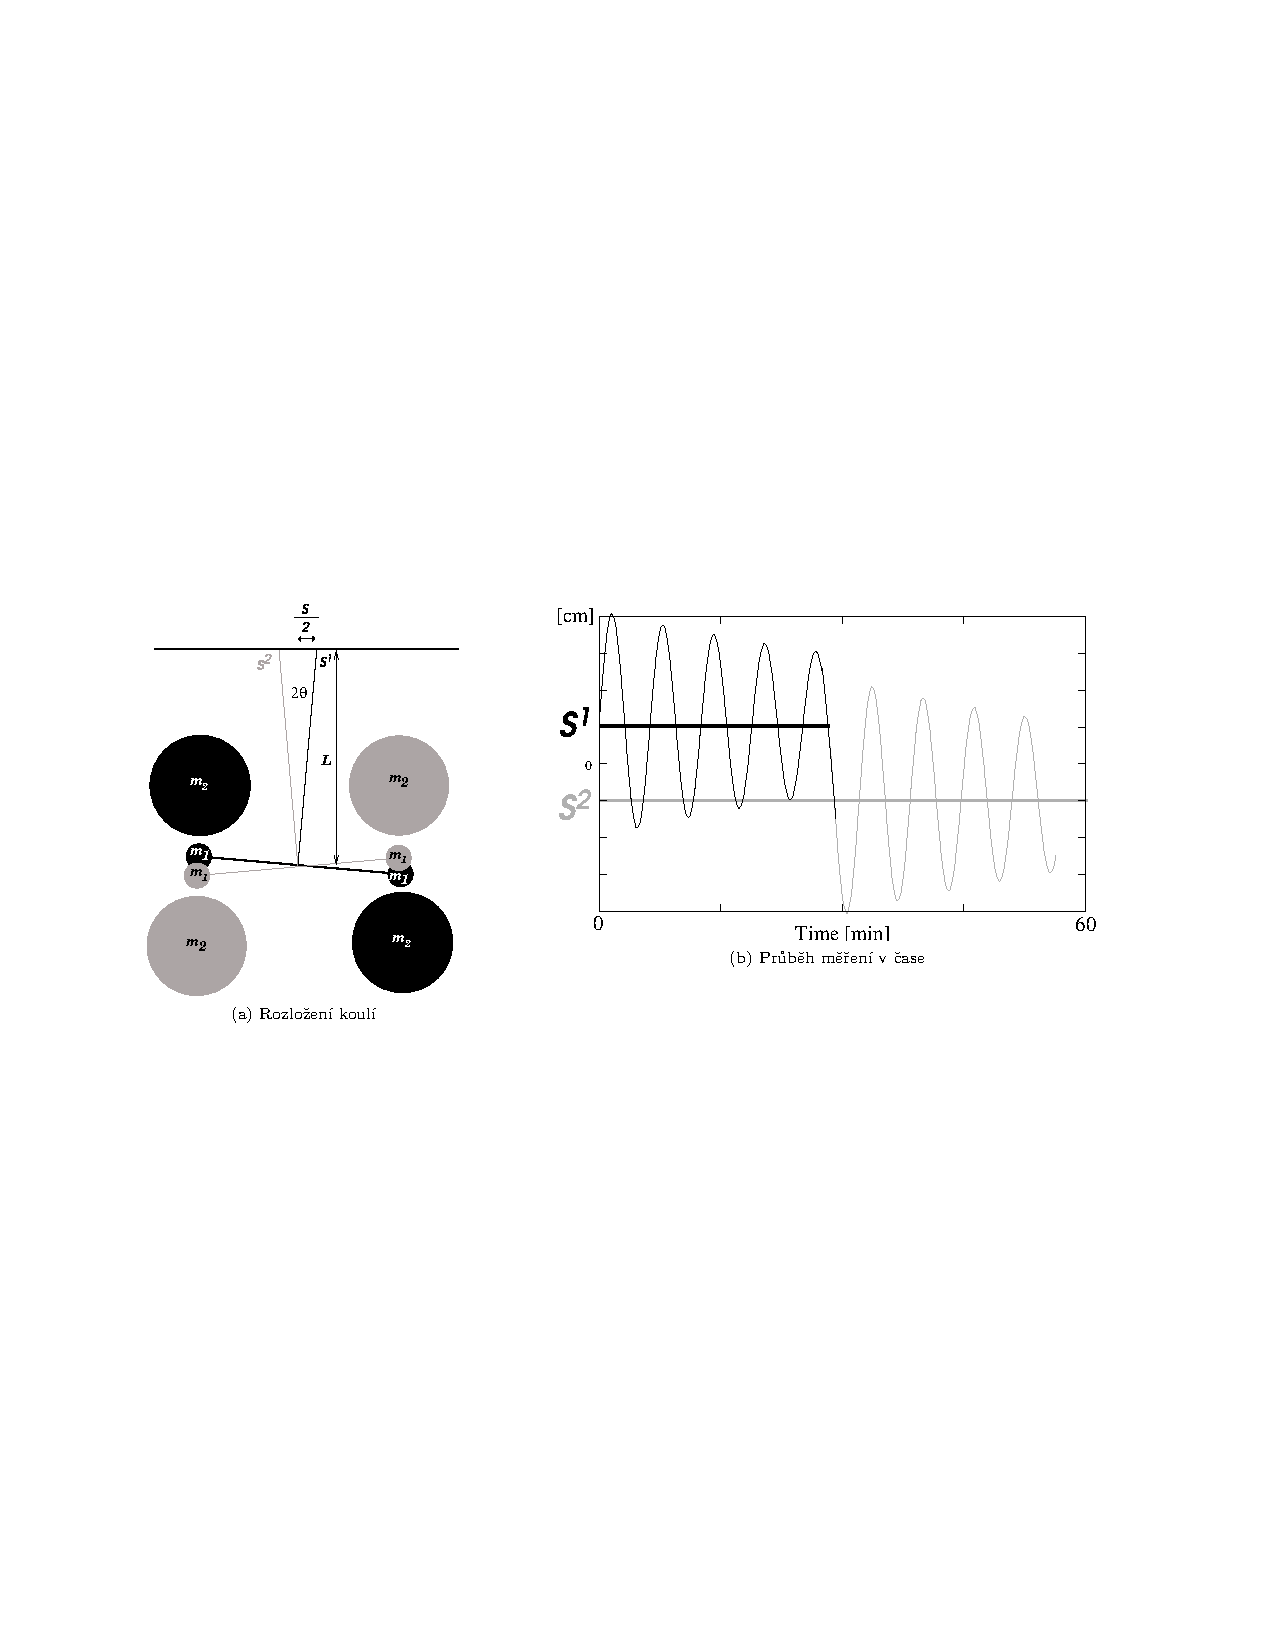
\includegraphics[width=\linewidth]{att/obr2.pdf}
						\caption{Schéma zapojení z \cite{bib:zadani}.}
						\label{fig:schema_2}
							    	
						
				\end{center}
			\end{figure}
	

\clearpage
\subsection{Grafy}

	\begin{figure}[h!]
	\begin{center}
	\vspace*{-1.5cm}
	    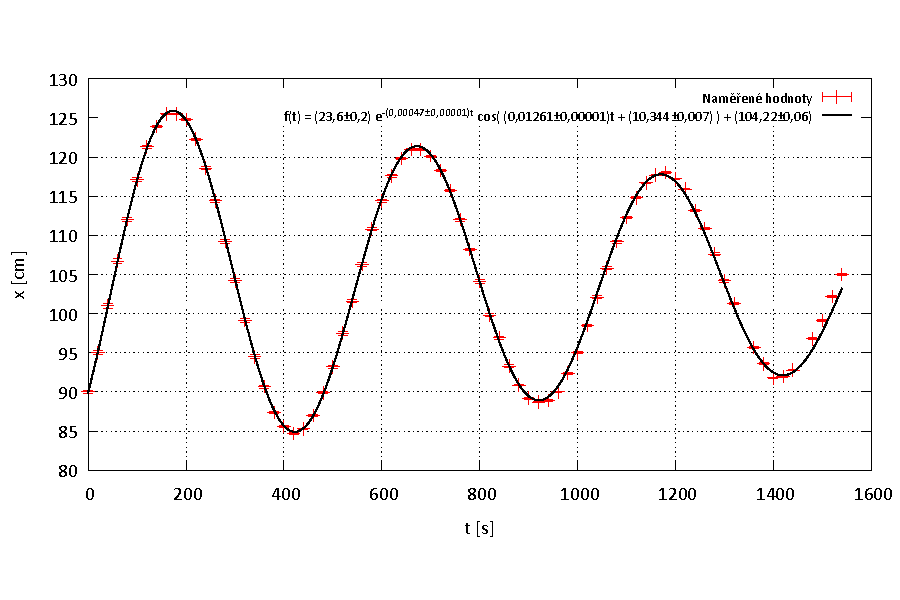
\includegraphics[width=\linewidth]{../gnuplot/data_1.pdf}
	    \vspace*{-1.5cm}
	    	\caption{Graf závislosti pozice $x$ na čase $t$ při měření v první poloze. Proložením funkcí pro tlumené harmonické kmity (\ref{eq:fitfce}) jsme určili periodu a rovnovážnou polohu.}
			\label{fig:g_1}
	\end{center}
	\end{figure}

	\begin{figure}[h!]
	\begin{center}
	\vspace*{-1.5cm}
	    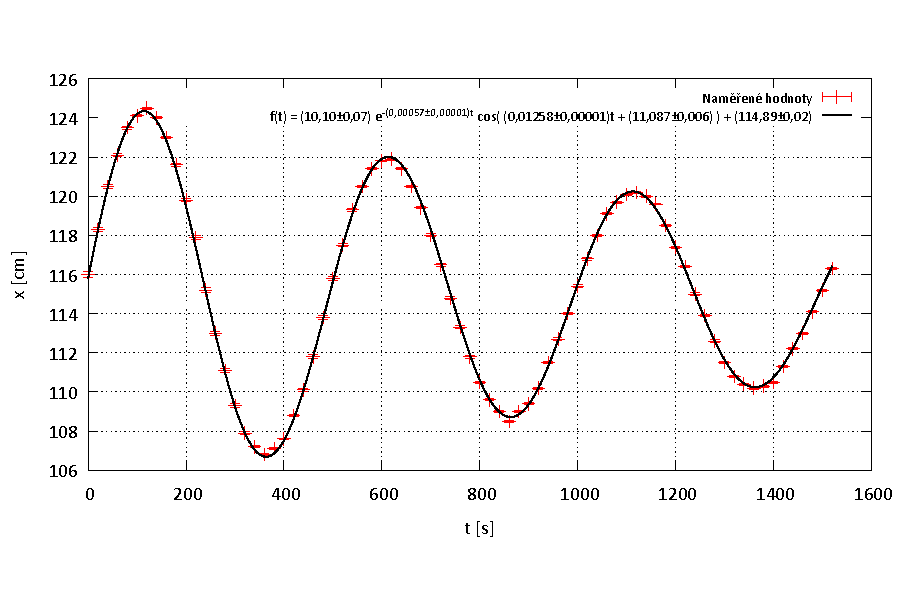
\includegraphics[width=\linewidth]{../gnuplot/data_2.pdf}
	    \vspace*{-1.5cm}
	    	\caption{Graf závislosti pozice $x$ na čase $t$ při měření v druhé poloze. Proložením funkcí pro tlumené harmonické kmity (\ref{eq:fitfce}) jsme určili periodu a rovnovážnou polohu.}
			\label{fig:g_2}
	\end{center}
	\end{figure}

	
% --- Konec dokumentu --------------------------------------------------


\end{document}

